\documentclass[10pt]{article}
%%%\documentclass{article}
%%%\usepackage[2-16]{pagesel}
%\usepackage[english,spanish]{babel}

\usepackage{times}
\usepackage{cite,verbatim,rotating}
\usepackage{subfigure}

\usepackage[paper=letterpaper,margin=1in,ignorefoot,ignorehead]{geometry}

%\usepackage{fullpage,setspace}
\usepackage{url}
%\usepackage{algorithmic}
%\usepackage{algorithm2e}
\usepackage{amsfonts}
\usepackage{amssymb}
%\setcounter{tocdepth}{3}
%\usepackage{simplemargins}
\usepackage{graphicx}
\usepackage{wrapfig}
%\usepackage{amssymb}
\usepackage{amsmath}
%\usepackage[dvips]{graphicx}
%%% remove comment delimiter ('%') and specify parameters if required
%\usepackage[dvips]{graphics}
%\setallmargins{1.0in}

\makeatletter
\renewcommand\section{\@startsection{section}{1}{\z@}%
                                    {-0.5ex \@plus -1ex \@minus -.2ex}%
                                    {1.0ex \@plus.2ex}%
                                    {\normalfont\Large\bfseries}}
\renewcommand\subsection{\@startsection{subsection}{2}{\z@}%
                                     {-0.5ex\@plus -1ex \@minus -.2ex}%
                                     {0.5ex \@plus .2ex}%
                                     {\normalfont\large\bfseries}}
\renewcommand\subsubsection{\@startsection{subsubsection}{3}{\z@}%
                                     {-0.5ex\@plus -1ex \@minus -.2ex}%
                                     {0.5ex \@plus .2ex}%
                                     {\normalfont\normalsize\bfseries}}
\renewcommand\paragraph{\@startsection{paragraph}{4}{\z@}%
                                    {-0.5ex \@plus -1ex \@minus.2ex}%
                                    {-2em}%
                                    {\normalfont\normalsize\bfseries}}
\renewcommand\subparagraph{\@startsection{subparagraph}{5}{\parindent}%
                                       {0.5ex \@plus1ex \@minus .2ex}%
                                       {-1em}%
                                      {\normalfont\normalsize\bfseries}}
\makeatother

\setlength{\abovedisplayskip}{2pt plus 2pt minus 2pt} \setlength{\belowdisplayskip}{2pt plus 2pt minus 2pt}
\setlength{\abovedisplayshortskip}{0pt} \setlength{\belowdisplayshortskip}{\belowdisplayskip}
\setlength{\itemsep}{0pt}

\setlength{\textfloatsep}{2 mm} \setlength{\dbltextfloatsep}{0 mm}
\setlength{\parindent}{0mm}
\setlength{\parskip}{0.4mm}

\newcommand{\mypage}[1]{\renewcommand{\thepage}{#1-- \arabic{page}}
\setcounter{page}{1}}

\renewcommand{\figurename}{Fig.}

%\renewcommand{\thesubfigure}{\figurename\ \thefigure.\alph{subfigure}}
%\makeatletter
%\renewcommand{\@thesubfigure}{\thesubfigure:\space}
%\renewcommand{\p@subfigure}{}
%\makeatother

\renewcommand{\baselinestretch}{0.940}
%%%%%%%%%%%%%%%%%From RANDY
\newcommand{\sens}{z}
\newcommand{\comnbrs}{{\mathscr{S}}}
%\newcommand{\physnbrs}{{\cal X}^{\text{phys}}}
\newcommand{\sensnbrs}{{\mathscr{X}}}
\newcommand{\metastate}{{\mathscr{Y}}}
\newcommand{\R}{{\ensuremath{{\mathbb{R}}}}}
\providecommand{\norm}[1]{\lVert#1\rVert}
\newcommand{\environ}{{\mathscr{E}}}

%\usepackage[pdftex]{graphicx}
%\vfuzz2pt % Don't report over-full v-boxes if over-edge is small
%\hfuzz2pt % Don't report over-full h-boxes if over-edge is small
%
\DeclareGraphicsExtensions{.jpg,.pdf,.mps,.png,.eps} %For pdftex

\newtheorem{definition}{Definition}[section]
\newtheorem{property}{Property}[section]
\newtheorem{corollary}{Corollary}[section]
\newtheorem{propose}{Proposition}[section]
\newtheorem{theorem}{Theorem}[section]
\newtheorem{lemma}{Lemma}[section]
\newtheorem{example}{Example}[section]

\DeclareMathOperator{\Cov}{Cov}
\providecommand{\abs}[1]{\lvert#1\rvert}
\providecommand{\norm}[1]{\lVert#1\rVert}
\newcommand{\E}{\ensuremath{\mathcal E}}
\newcommand{\F}{\ensuremath{\mathcal F}}
%%%%%%%%%%END FROM RANDY%%%%%%%%%%%%%

\usepackage{fancyhdr}
\setlength{\headheight}{12pt} \pagestyle{fancy}

%%%\fancyhf{} \lhead{\small Project Description} \rhead{\footnotesize
%%%CPS:Large:Collaborative: {\bf CASAP} -- Context-Aware Systems for
%%%Agricultural Practices} \cfoot{\thepage}

%%%\small
\fancyhf{}
%\lhead{Context-Aware Management of Heterogeneous Sensor Networks}
%%%\lhead{\small Project Description}

%\rhead{\footnotesize CPS:Frontiers:Collaborative Research:Dynamic Entanglement of Control and Data Management in Precision Agriculture} \cfoot{\thepage}

\rhead{\footnotesize Dynamic Data-Driven Networks of Cyber-Human Internet of Things for Smart and Connected Communities} \cfoot{\thepage}

\normalsize

\newcounter{taskcount}

\setcounter{taskcount}{0}

\newenvironment{task}
{% This is the begin code
\refstepcounter{taskcount} \textbf{\underbar{Research Tasks Group
(RTG)-\arabic{taskcount}:}} \itshape }
{% This is the end code
}

\renewcommand{\thetaskcount}{\textbf{RTG-\arabic{taskcount}}}

\newenvironment{plan}
{% This is the begin code
\textbf{\underbar{Proposed Approaches:}}} {}

\begin{document}

%\flushbottom

%%%\pagestyle{empty}
\mypage{Project Description }

\section{Introduction}\label{intro}%%

According to IDC (www.idc.com) -- a global provider of market intelligence, advisory services, and events for the information technology, telecommunications and consumer technology markets -- the worldwide shipment of smart connected devices will surpass 2.5 billion units in 2017. As the cost, size, and power requirements keep decreasing, computing will be embedded in all kinds of products and everything that can benefit from the Internet will be connected. Not only stations, computers or laptops, but also tablets, smartphones, cars, game consoles, TV sets, cameras, machines, lights, locks, and home appliances.\\

People and data are already online. Soon, all sort of things with sensors, actuators and places will be also online. All sectors of activity will benefit from applications that leverage the interconnection of embedded systems with IT systems. Intelligent transport solutions can speed up traffic flows, reduce fuel consumption, and safe lives. Smart farming solutions will improve the production and delivery of safe and healthy food. Remote health monitoring will provide convenient access to healthcare, raises it quality, and save money. Utilities management, education, government services, retail sectors etc.… all will also benefit from such couplings and the things will leave across all different systems. \textbf{The next step is to interconnect these individual systems into a system of systems, and here we are confronted to such a scale and heterogeneity that we are reaching a limit in networking and software engineering}.\\

In this project, we aim to investigate issues related to the design and development of a secure physical and computational networked environment, consisting of billions of connected smart objects (things), which allows interoperability and facilitates efficient collection and processing of data and analytics. These smart objects may come from diverse environments such as smart appliances at homes, smart mobile surveillance system such as fire trucks and police cars, smart transportation entities (e.g., cabs or buses), etc. By establishing a dynamic instantiations of Internet of Things (IoT) structures, we aim to  provide an automatic resource optimization and other intelligence into these evolving collections of smart connected objects. However, rather than endowing them with autonomously cognitive chips, we ask for manufacturers, retailers and users/owners, through an established social network of things, to elaborate finely tuned dispatches to be distributed toward the smart objects through middleware fogs located in the individual homes. \\

Nowadays, existing start of the art related to the design of IoT systems is highly compartmentalized, the data collection and analytics processing across a variety of heterogeneous IoTs has limited support, and the interoperability of objects across domains has not been addressed at a level that would provide the kinds of optimizations that this project aims.. In this project, we introduce the concept of collaborative Social Network of Things that would enable data and analytics sharing across objects that exhibit similar operating characteristics and/or have similar profiles in terms of usage and user/manufacturer parameters. In addition, we propose to develop a hierarchical middleware implemented as fogs to allow interoperability with context-aware security properties associated with different nodes. These middleware fogs, mainly implemented in smart boxes/gateways within local networks, will manage the communication between the associated smart objects and the network in an optimized way that takes into account both the characteristics of the smart objects and the preferences of the users. The massive generated data by all these connected smart objects and stored in the system will enable the cognitive network, through deep learning algorithms, to raise dynamic procedures that will enable a multi-criteria optimizations of the  behavior  of these smart objects.\\

A typical scenario could be as follows. During his  coffee break at the office, Jack decides to lower by 5 degrees the set point temperature of his home heating system – which must go into action when he is less than 1 mile from his home and in any case no later than 6PM. However, if the outside temperature drops below certain threshold, the temperature must go up by 5 degrees. At lunchtime, a colleague of his gives Jack a list of instructions corresponding to a new method for washing wool sweaters; he  sends the file directly to his home through the social network where a service will adapt the instructions to that washing machine’s particular technical features and his personal preferences for extra soft cloths. Back at home, Jack launches “my angry day” profile through  smartphone, which automatically dims the light and has the Hi-Fi play his favorite relaxing music. Meanwhile, a tip from the network tells Jack to turn off all TVs to avoid getting further depressed. During the night the washing machine starts the cycle at the time the electric company informs it to be the most favorable.\\

While the above describes a single user, what we aim to investigate in this project is how to incorporate multiple users and smart devices into multiple instances of Social Network of Things, that can be generated/organized and dissolved on-the-fly; where different criteria can be used to orchestrate the behavior of (groups of) instances subject to multiple constraints; and certain security and privacy concerns are ensured. In the context of “Jack” scenario, this would mean collaboratively regulating the temperature with other units in Jack’s building; collaboratively deciding about the cycle of the washing machine in terms of optimizing the grid-demand within a city-block; adjusting the Hi-Fi themes based on the fact that Jack decided to join his co-workers for a happy-hour; etc… Moreover, we plan to provide novel data analytics methodologies that will: (a) incorporate the fact that some users may not be cooperative in terms of suggested regime of use for certain devices/task; (b) provide a specific behavioral insights to be used by various manufacturers when planning the design of certain devices so that they can be better adapted to changing conditions of use. 
The architecture we target to support such  scenarios is depicted in Figure 1. We aim at providing methodologies and tools for two basic modes: \\

\begin{wrapfigure}{R}{0.30\textwidth} \vspace{-3mm}
	\centerline{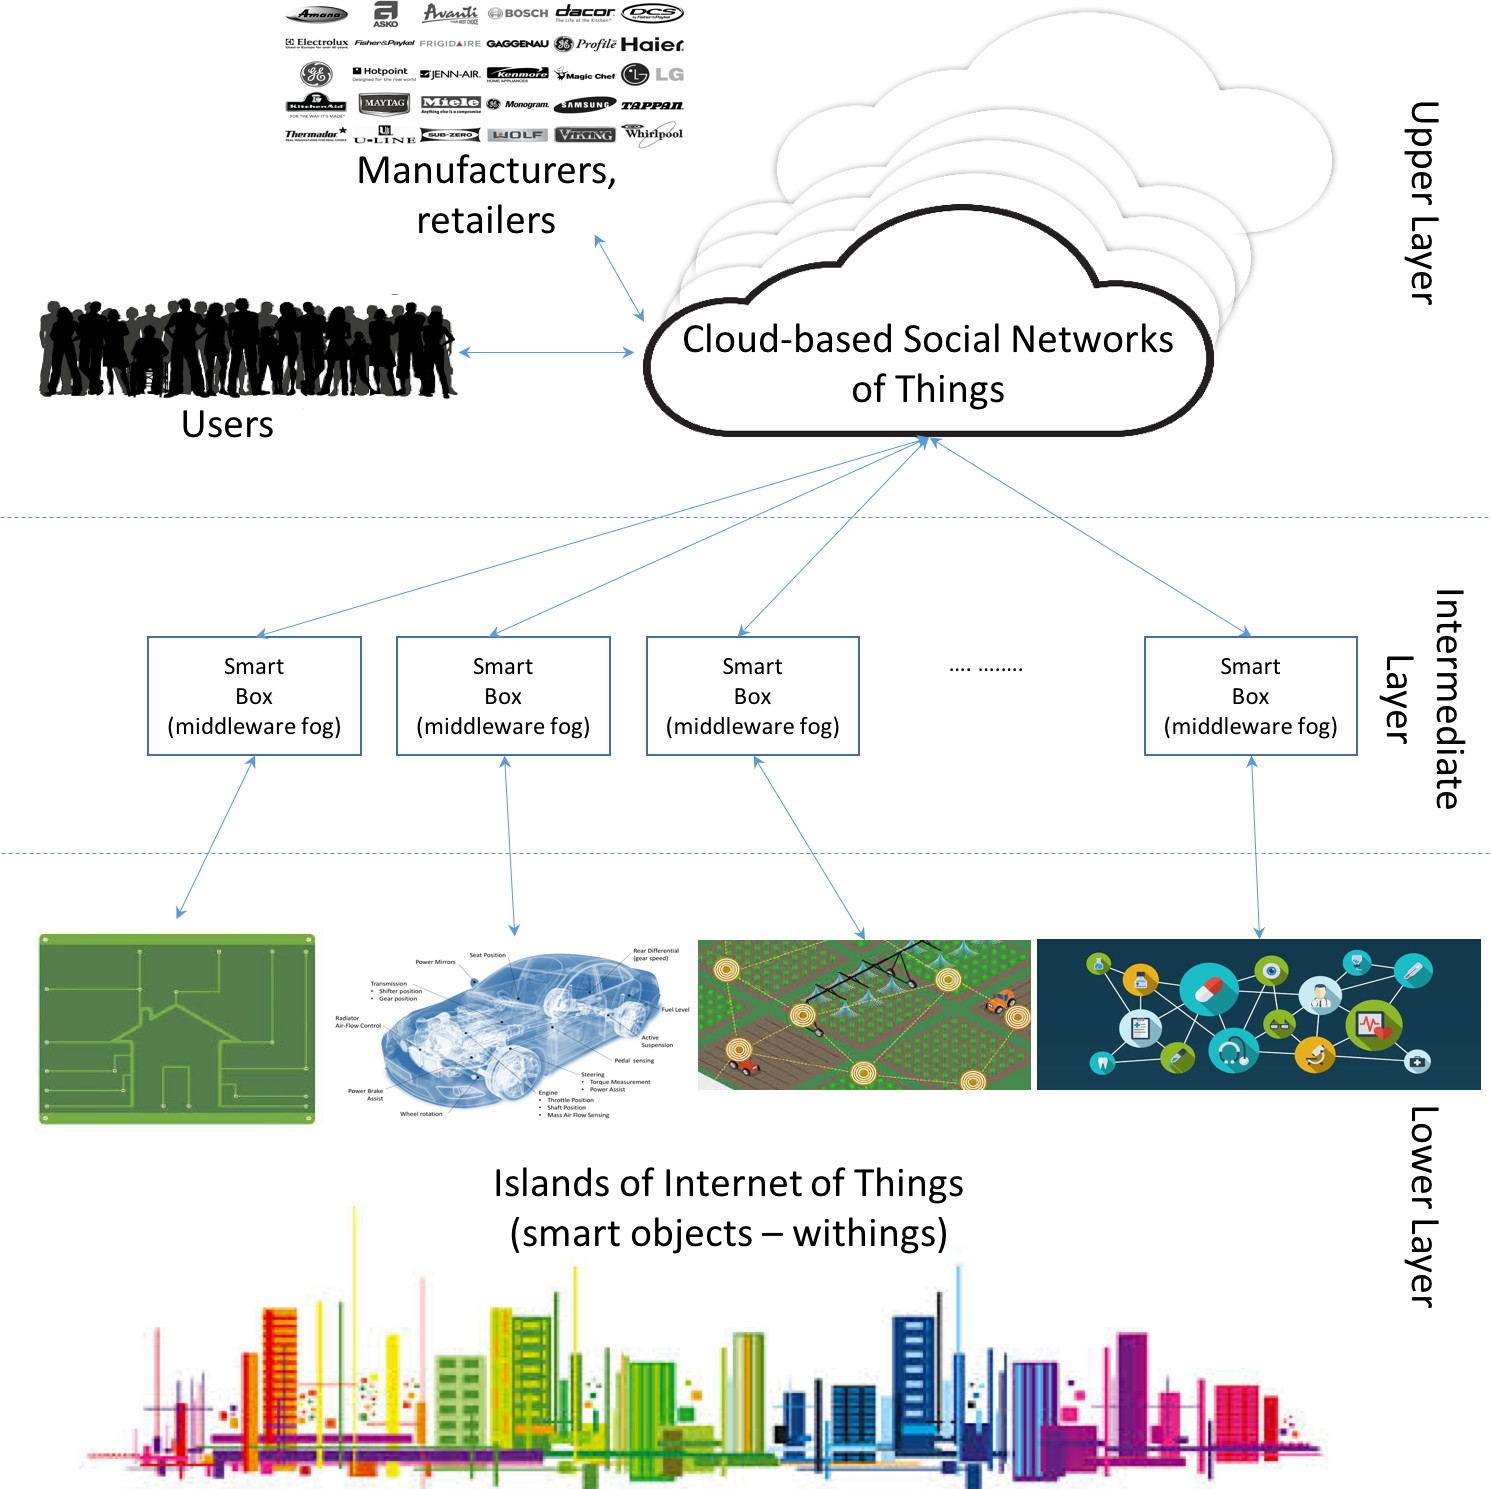
\includegraphics[width=0.30\textwidth]{./fig1.png}}
	\vspace{-3mm} \caption{\small An overview of the system}
	\label{fig1}
	\vspace{-3mm}
\end{wrapfigure}

(1)  The first setup consists of a set of middleware fogs, located in each smart box/gateway of a smart home or public area, grouped together in a social network along with profiles of manufacturers, retailers and users/owners. The lower layer is formed by all the real devices/objects (things), such as a fridge, a washing machine, a heater, a TV, a Hi-Fi, etc., where each one is abstracted by what we refer to as WiThing (WiT) for Wireless Thing. The WiT is the first level of the device abstraction and its role is to (1) uniquely identify an object/device worldwide, (2) represent the object in terms of its properties/functionalities through an MIB (Management Information Base), and (3) constitute a bidirectional interface for all communications between the object and the middleware fog located in the smart box/gateway. The intermediate layer contains the smart box/gateway where the middleware fog is implemented. The latter is composed of an ensemble of interconnected modules that will govern all the requests issued by the user through a proper front-end application. To this end, this smart box must interface with any object/device it meets in the surroundings, i.e., any virtual device communicated by the real objects/devices. The upper layer contains the social networks of manufacturers, retailers and users/owners with the generic representations (avatars) of their objects/devices. It consists of a large database with an enquiry system based on sophisticated algorithms.
Throughout this complex environment, and in order to fully automate the deployment and control of such Internet of Things, gathering of important data, identification of correlations in this chain of complex events, and triggering the required responses, a plethora of issues in data collection and processing (storage/retrieval, querying and information fusion), knowledge discovery, and security and privacy need to be investigated in unified framework. We assert that  such integrated large scale effort, involving researchers from diverse backgrounds, is necessary to  enable exploiting the full potential of the Internet of Things technology  and make it ubiquitous of use.\\

(2) The second setup complements the previous one in terms of inter-contexts couplings and dynamic formations (and dissolution) of corresponding Avatars. In terms of notation in Figure 1. it is best explained by the following scenarios:
(a) If we have a collection of Avatars corresponding to a particular device (e.g., a washer) in a collection of residential units, depending on the geographical context we may want to form different instances of (meta)Avatars corresponding a group of same devices but operating in: (i) a group of houses in a suburban residential area; and/or (ii) a group of buildings in a near-downtown area.
(b) Complementary to this, the Avatars corresponding to washers in different units in an apartment complex, may be tied with the Avatars corresponding to entertainment devices in the same and/or neighboring buildings.
(c) The collection of Avatars representing the traffic-density in different geographical regions may be tied with the crime-rate in those and/or near-by regions and with the ones corresponding to activities of electronic devices in the police cars. However, after a certain time of the day/night, such (meta)Avatars may cease to exist. 

The situational awareness that we aim to capture by dynamically creating Meta-Avatars is illustrated in Figure 2. We note that, in addition to the scenario-oriented discussion above, the Meta-Avatars may be created based on:\\

\begin{wrapfigure}{R}{0.30\textwidth} \vspace{-3mm}
	\centerline{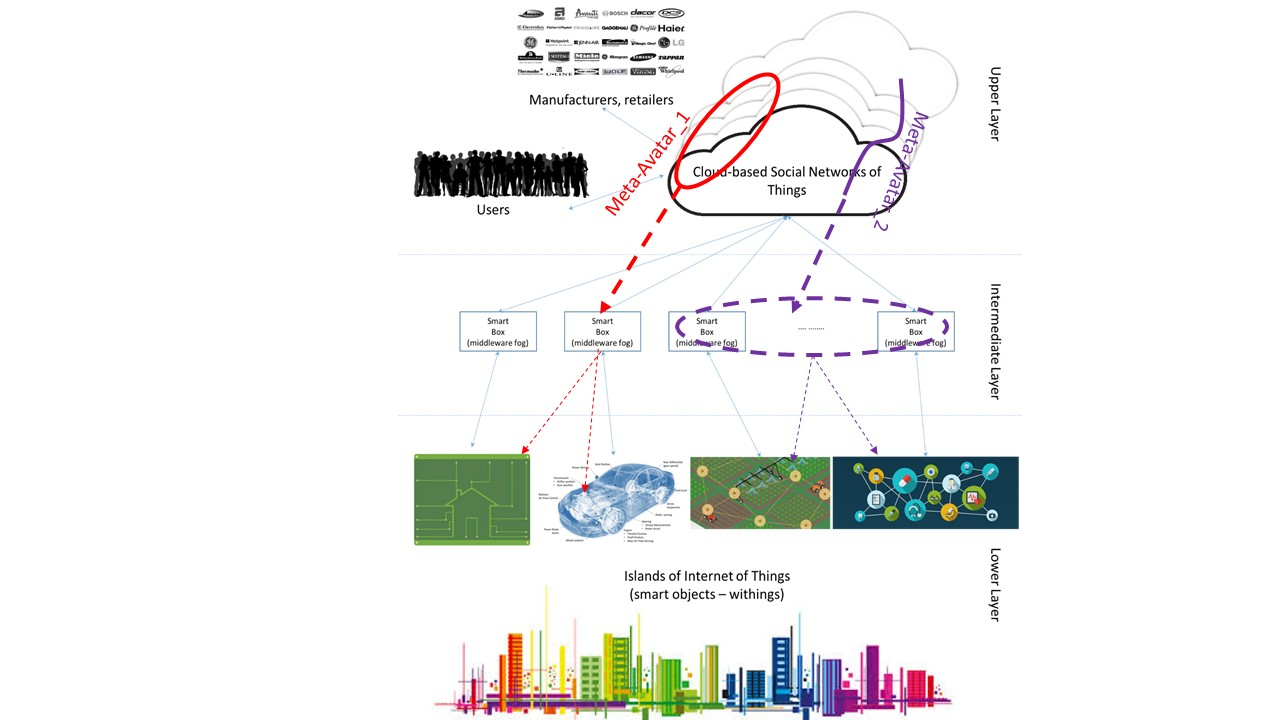
\includegraphics[width=0.30\textwidth]{./fig2.jpg}}
	\vspace{-3mm} \caption{\small Meta-avatars}
	\label{fig1}
	\vspace{-3mm}
\end{wrapfigure}

-	Particular cyber-properties: e.g., status of network infrastructure, privacy constraints, etc.
Logical or semantical properties which may entail dynamically forming (and dissolving) hierarchies of such avatars.\\

The main Intellectual Merits of the proposed project are:
----Repeat the Intellectual Merits here…


\section{State of the art}\label{soa}
We now present an overview of the state of the art, both from the perspective of the current properties of devices and networking technology features, as well as from the perspective of related works in several fields that, in one way or another, may be used to achieve our objectives – however, the fall short of several important aspects.

\subsection{Whatever Proper title of this sub-section}
The vast majority of devices are endowed with electronic interfaces, made of buttons and the like, inviting users to operate selections from among a limited set of options pre-featured by the manufacturers. They may concern options, such as, ventilation on/off button in an oven, a selection of delicate option in a washing machine, air-condition on/off button in a car, and so on. While these older devices are considered somehow efficient and simple, the trend is towards more technological and ubiquitous devices.
The operational innovation of our approach is to make a move of the interface a step ahead and a step farther so as to realize a deep, remote and smart control. In this case, the manufacturer makes all/most of the operational parameters, such as spin speed and duration, totally manageable and configurable by the user. In turn, the user drives these parameters via software, hence makes them obeying to automatic procedures/instructions that have been elaborated and optimized in advance, with the help of the manufacturer, other contributors, and/or the networked intelligence.
Thus, we need to have this new hardware/software interface managing signals/data back and forth between actuators/sensors and a logic unit with the result of detaching the user from any physical contact with the device (thing). To this end, in the project we will use open source electronic boards, such as Arduino boards (https://www.arduino.cc/), Parallella boards (https://www.parallella.org/) and/or Raspberry-Pi boards (https://www.raspberrypi.org/). They are powerful prototyping boards based on flexible, open and easy-to-use hardware and software. These devices are wirily and/or wirelessly connected to the Internet from which they can be easily visible and accessible. We foresee that their exploitation will lead microelectronic companies to develop specific chips for a massive diffusion of this new technology in a near future.
In order to realize the vision of an Ambient Intelligence in a future network and service environment, heterogeneous wireless sensor and actuator networks have to be integrated into a common framework of global scale and made available to services and applications via universal service interfaces \cite{SSR05}. The goal is to reach a distributed open architecture with interoperability of heterogeneous systems, neutral and easy access, clear layering and resilience. It should provide the necessary network and information management services to enable reliable, secure and accurate interactions with the physical environment.
The idea is to provide an integrated platform that offers unified data access, processing and services on top of existing ubiquitous services of the Internet of Things to integrate heterogeneous sensors/actuators in a uniform way. From an application perspective, a set of basic services encapsulates sensor/actuator network infrastructures hiding the underlying layers with the network communication details and heterogeneous sensor hardware and lower level protocols.

A heterogeneous networking environment indeed calls for means to hide the complexity from the end-user, as well as applications, by providing intelligent and adaptable connectivity services, thus providing an efficient application development framework. To face the coexistence of many heterogeneous set of things, a common trend in Internet of Things applications is the adoption of an abstraction layer capable of harmonizing the access to different devices with a common language and procedures \cite{ERA09}. Standard interfaces and data models ensure a high degree of interoperability among multiple systems. However, typical drawbacks of misconfigurations and traffic congestions are normally exasperated by the node heterogeneity. These drawbacks will be overcome in the project through the adoption of islands architecture. On the one hand, smart gateways in their locations will hide all the complexities of the underlying standards. Hence, wireless connections of the devices/machines to the web/Internet, using communication technologies like Zigbee \cite{Zigbee12}, Z-wave \cite{Zwave12}, Wi-Fi \cite{Wifi}, plus the mapping of every device to a unique ID, will provide full, intelligent and secure control over it. With these smart boxes/gateways, technological limitations will completely disappear and the devices will become identifiable only through their functionalities with clear and consistent APIs. On the other hand, the middleware fog constitutes an abstraction level where all the devices, viewed as entities sharing their functionalities (avatars), are transparently managed and used. The goal is to manage the collaboration between heterogeneous devices through a simple API level in conjunction with the mentioned communication protocol able to reach the peer within the location singularly.
Most existing solutions for middleware adopt in general a service-oriented design tailored mainly to support a network topology of sensors that is both unknown and dynamic. But while some projects focus on abstracting the sensors in the network as services (such as in HYDRA \cite{ZH09, ERA10, ZH08}, SENSEI \cite{PBEV09}, SOCRADES \cite{GTKSS10}, and COBIS \cite{cobis07}), other projects devote more attention to data/information abstractions and their integrations with services (among which are SOFIA \cite{HLBT10}, SATware \cite{MDMV09}, and Global Sensor Networks GSN \cite{AHS07}). A common thread throughout all of these solutions, however, is that they handle the challenge of an unknown topology through the use of discovery methods that are largely based on the well-known traditional service/resource discovery approaches of the existing Internet, ubiquitous environments and wireless sensor and actuator networks \cite{AM08, ZMN05, MRPM08}. For instance, SOCRADES provides discovery on two levels, the sensor level and the service level, which can employ either standard web-service discovery or a RESTful discovery mechanism (for RESTful services). COBIS, on the other hand, uses its own service description language COBIL 2 (Collaborative Business Item Language), where service functions and keywords are annotated with a verbal description.
Another point of agreement in the state-of-the-art of middleware solutions is in the widespread use of semantics and metadata to overcome heterogeneity challenges. Indeed, it is standard practice to use ontologies to model sensors, their domains, and sensor data repositories [7, 18, 19]. Some projects even go a step further and also include context information [9], or service descriptions [6, 7, 8]. And as a type of service composition, many projects support the concept of virtual/semantic sensors (for instance, in HYDRA, GSN and SATware), i.e. entities that abstract several aggregated physical devices under a single service. A different implementation of a similar idea, though, is provided in the SATware project, where virtual sensors actually correspond to transformations applied to a set of raw sensor streams to produce another semantically meaningful stream.
Regarding scalability, most projects address this challenge by pursuing modifications in the underlying sensor/actuator network topology. Sometimes, this is done by adopting fully-distributed infrastructures (such as in COBIS and SOFIA), and sometimes through an architecture of peer-to-peer clusters (e.g., GSN). In our view, however, while these approaches work well for the existing Internet, where traffic is made up of a relatively small amount of service interactions, they will not fit for the complex weave of interactions that will be commonplace in the Internet of Things. In the Internet of Things, a large number of requests will involve intricate coordination among millions of things and services, whereas on today's Internet most requests are largely point-to-point. Therefore, the number of packets transmitted in the network will grow strongly and nonlinearly as the number of available services increases. In such an environment, performing even a simple service discovery may exceed acceptable time, processing, and memory constraints. //NOTE: the last paragraph needs to be tied (cf. (2)/Fig.2 in the intro with the problems related to “Possible Worlds Semantics�� and the efficient pruning the needs to be performed

\subsection{Data and Process Integration}
Heterogeneous data integration is a topic which, in addition to the database community broadly \cite{Cohen98,HalevyRO06}, has also been investigated by more specialized research foci: -- bioinformatics \cite{KirstenR06,MostafaviM10}; information management and text retrieval \cite{CouletGDAMS11,HammerGIPUW95,Torlone08}; sensing/actuation and tracking \cite{AvciTS16,ChawatheKRS04,SalarianCN12} (to name but a few). While the role and the impact of the semantics have been recognized and addressed \cite{BergamaschiCVB01,CastanoFMR04}, the existing results still have limited cross-contextual support. For instance, the works investigating the benefits of semantics for resource discovery (cf. \cite{CastanoFMR04}) do not take into consideration the role of different devices that may enter and/or leave a particular geo-social� network dynamically, as well as their impact on real-time adjustments (as well as the impact of their cessation).
To-Do – Goce:
Overview of:

a.	Data integration + distributed query processing; workflows~\cite{LiCLWPZB12,PandeyB12,PoolaRB16}; Wireless Actuator Networks

b.	Analytics and platforms in-context (Cloud/Hadoop; NoSQL; Warehousing)~\cite{ToosiCB14}


\section{Proposed research overview}\label{research-overview}
We now proceed with identifying the main challenges that the proposed project will address, with a brief overview of the proposed research tasks (research challenges), followed by an introduction of the team and their expertise.


Research Challenge 1 (RC-1): Data collection and processing
…



Research Challenge 2 (RC-2): Knowledge discovery
…


Research Challenge 3 (RC-3): Security, privacy (anonymity) and trust

The Internet of Things is foreseen to bring a multitude of services with a vision of creating a smart self-configuring and interconnected world for the benefit of end users. With the extensive research and development of computer, communication and control technologies, it is possible to connect all things to the Internet such that the so-called Internet of Things (IoT) can be formed. These things may be equipped with devices such as sensors, actuators, and tags, in order to allow people and things to be connected anytime and anywhere, with anything and anyone. IoT will enable collaborations and communications among people and things, and among things themselves, which expand the current Internet and will radically change our personal, corporate, and community environments. However, a plethora of security, privacy, and trust challenges need to be addressed in order to fully realize this vision [20, 21, 22, 23]. When more and more things connect to the Internet, security and privacy issues become more serious, especially in the case that these things are equipped with actuators and can support control.
For better protection of secure communication and user privacy, including location, identity and behavior habits, it is necessary to develop anonymous communication theories, methods and key technologies of anonymous communication systems in all varieties of application environments. Anonymous communication is used to hide communication participants or communication relations to achieve effective protection for network nodes and user identities. Anonymous communication can address potential network security issues, and becomes one of the hot topics in the field of network and information security. With reference to security, data anonymity, confidentiality, and integrity need to be guaranteed, along with providing authentication and authorization mechanisms in order to prevent unauthorized users (i.e., humans and devices) to access any system. Concerning privacy requirement, both data and user personal information have to be confidentially manipulated since devices may manage sensitive information (e.g., user habits, locations, etc). Finally, trust is also a fundamental issue since the IoT environment is characterized by multiple devices that have to process and handle the data in compliance with user needs and rights.
To realize a trusted, secure, and privacy preserving social network of things, we plan to address in this proposal the following security, privacy, and trust management related tasks:

T-3.1: Define a new scheme of anonymizing things and representing them as avatars in the social network of things.

T-3.2: Authentication of data collected in fogs in the presence of malicious attackers, despite the attack surface being very broad, ranging from PHY layer to application layer.

T-3.3: Achieving end-to-end secure and privacy-preserving information flow monitoring between users and things, covering all sort of things and access networks using physiological and physical layer properties.

T-4.3: Design of secure, fast and friendly authentication schemes to allow users of the social network of things to access the data of interest through diverse mobile devices such as smartphones and tablets.

\section{Research tasks}\label{research-tasks}
We now proceed with a detailed presentation of the main research of the proposed project. 


\subsection{Data collection and processing} 
(Goce + Mubbasir)\\
Data cleaning, data collection, sharing, processing, analytics\\
How can we secure the collected data and how to make it available?\\
APIs and libraries for building applications 




\paragraph{Knowledge Representation and Reasoning} 

The processed data from above will be represented as a set of discrete time series, or \emph{fluents} which encode the states and properties of different \avatar which change over time. \todo{give example}. To facilitate efficient reasoning and knowledge discovery in a dynamic smart and inter-connected system of avatars, we will consider a level of abstraction, termed as \emph{events }. Events constitute meaningful interactions between two or more \avatar and serve as the basis for identifying relationships between them towards creating social networks of avatars. \todo{give example}. We define the specific terms and concepts we will use for event-centric knowledge representation and reasoning below. 

\noindent \textbf{Smart Avatars} The notion of smart objects~\cite{Kallmann:1999:DIS:323663.323683} has been popularly used in the graphics and animation community to embed intelligence and semantics in virtual objects. We extend this formalism to represent both IoT objects as well as IoT users. This unified formalism allows us to seamless consider sensors, controllers, actuators, and human users within the same social community.  We define a smart avatar $\smartobj{} \in \world$ as $\smartobj{} = \langle \affordances, \state{} \rangle$ with a set of advertised affordances $\affordances$ and a state \state{}. An affordance $\affordance(\affordanceowner, \affordanceuser) \in \affordances$ is an advertised capability offered by a smart avatar that manipulates the states of the owner of an affordance $\affordanceowner$ and a smart avatar user $\affordanceuser$. 

\noindent \textbf{State.} The state $\state{} = \langle \attributeSymbol, \relationshipSymbol \rangle$ of a smart object $\smartobj{}$ comprises a set of attribute mappings \attributeSymbol (fluents), and a collection of pairwise relationships $\relationshipSymbol$ with other avatars. With this representation, we can make logical inferences between objects using a declarative PROLOG-like knowledge reasoning engine. 
%An attribute \attributemapping{i}{j} is a bit that denotes the value of the $j^{th}$ attribute for $\smartobj{i}$. 



%A specific relationship $\relationship{\cdot}{\cdot}{a}$ is a sparse matrix of $|\world| \times |\world|$, where \relationship{i}{j}{a} is a bit that denotes the current value of the $a^{th}$ relationship between \smartobj{i} and \smartobj{j}. 


%\noindent \textbf{Rules.}  A rule $\Rule_x(i,j) \in \Rules$ between two smart objects \smartobj{i}, \smartobj{j} is true or false, depending on the states and relationships of both objects. Rules allow for logical inference between objects and are used for reasoning such as evaluating whether a character can access a particular room, or manipulate another smart object based on the current world state. They are defined and solved using a declarative PROLOG-like interface 

\noindent \textbf{Events.} Events are used to encode context-specific interactions between two or more smart avatars, and provide an appropriate level of abstraction for knowledge discovery  An event is formally defined as $\event{} = \langle \tree,  \precondition{}, \postcondition{} \rangle$. A precondition $\precondition{}: \groupState{\smartObjectGroup{}} \leftarrow \{\true, \false \} $ is a logical expression on the compound state \groupState{\smartObjectGroup{}} of a particular set of smart avatars $\smartObjectGroup{}: \{ \smartobj{1}, \smartobj{2}, \ldots \smartobj{|\roleSet{}|} \}$ that checks the validity of the states of each smart object. \precondition{} is represented as a conjunction of clauses $\clause{}{} \in \precondition{}$ where each clause \clause{}{} is a literal that specifies the desired attributes of smart objects, and relationships between pairs of participants. A precondition is fulfilled by $\smartObjectGroup{} \subseteq \world $ if $\preconditionFunction{\event}{\smartObjectGroup{}} = \true$. The event postcondition $\postcondition{} : \groupState{} \rightarrow \nextGroupState{}$ transforms the current state of all event participants \groupState{} to \nextGroupState{} by executing the effects of the event. We can extend this definition to model non-deterministic, fuzzy events with a probabilistic notion of success or failure. Events may optionally have a controller which defines the series of affordance activations within the smart avatars to produce its desired outcome. We represent this control logic using an extended version of Behavior Trees that facilitate parameterization. Parameterized Behavior Tree (PBT)~\cite{Shoulson:2011:PBT:2177817.2177835} are an effective model for representing coordinated control logic  between multiple smart avatars. 

PI Kapadia has extensive prior experience in developing event-centric knowledge bases for inference and reasoning in virtual worlds~\cite{Shoulson:2013:EPA:2522628.2522629,2015-fdg-bstl,Kapadia:2015:CAI:2699276.2699279,Kapadia:2016:CCN:2982818.2982846} which will be extended to represent the IoT domain. 


%ADAPT~\cite{Shoulson:2013:EPA:2522628.2522629}
%BSTL~\cite{2015-fdg-bstl,Kapadia:2015:CAI:2699276.2699279}
%behavior authoring~\cite{behaviorCGA,Kapadia:2011:BAC:1944745.1944779}
%story world~\cite{AIIDE1511583}
%CANVAS~\cite{Kapadia:2016:CCN:2982818.2982846}





%$\roleSet{} = \{ \role{i} \}$  define the desired roles for each participant. \role{i} is a logical formula specifying the desired value of the immutable attributes \attributemapping{\cdot}{j} for \smartobj{j} to be considered as a valid candidate for that particular role in the event.  


%An event instance $\instance = \langle \event, \smartObjectGroup{} \rangle$ is an event \event populated with an ordered list of smart object participants \smartObjectGroup{}.  $\preconditionFunction{\event}{\smartObjectGroup{}} = \true$. The event postcondition $\postcondition{} : \groupState{} \rightarrow \nextGroupState{}$ transforms the current state of all event participants \groupState{} to \nextGroupState{} by executing the effects of the event. When an event fails, $\nextGroupState{} = \groupState{}$. An event instance $\instance = \langle \event, \smartObjectGroup{} \rangle$ is an event \event populated with an ordered list of smart object participants \smartObjectGroup{}. 

%? which represent the specific values of avatar fluents at specific points. Events occur on a set of avatars which are the participants, and produce a change in state of these avatars which are defined as event postconditions. Events may additionally be pre-conditioned on the participant states to indicate what conditions must be satisfied in order for an event to successfully execute. 

This symbolic representation of avatars and theiry dynamic states in terms of key events will facilitate the development of an event calculus ? allowing us make inferences about the relationships and properties of these avatars using first and second-order logic. This reasoning will be used as the basis for knowledge discovery described in Section XX. Knowledge discovery will entail the identification of relationships between the properties of different avatars, clustering of avatar to create compound entities, and the discovery of salient events. 


 

\subsection{Knowledge discovery: social network of avatars (virtual world)}
(Ashfaq + Vladimir)

Tasks:
\begin{itemize}
	\item Build spatio-temporal avatar profiles
	\item Group avatars into groups according to similar profiles. I.e., construct social network of profiles and do graph clustering.
	\item Predict avatar behavior from group profiles
\end{itemize}


We will use Gaussian Process dynamic models (GPDM) as profiles. GPDMs can be used for both modeling isolated avatars and interactions between avatars.  We can use a framework similar to \cite{Shen2015-jr,Shen2015-ft,Shen2012-vi}.  Then extend using our trajectory refinement and optimization approaches \cite{yoon2016}.

However, we need to consider the fact that this system is heterogeneous, i.e., things and humans.  So should have a hierarchical model, one level for things, one for humans, then merge on higher level.


\subsection{Security, privacy and anonymity}



Security poses a great challenge for IoT. In addition to security threats common for networked systems in general, IoT systems are further confronted by the fact that they necessarily rely on wireless signals for communication. We propose to address challenges stemming from the \emph{physical layer} attacks on IoT systems. In particular, while Multi-User Multiple Input Multiple Output (MU-MIMO) systems are considered the ultimate next step in the wireless bandwidth race (because they leverage spatial multiplexing to send independent data streams to multiple terminals simultaneously, effectively improving spatial reuse), they could be utilized as an effective and sophisticated \emph{denial-of-service} tool. Indeed, by creating controlled signals in an area, it can selectively disrupt performance of Wi-Fi networks and sensors in an area, while still making it hard to detect or classify such behavior (precisely due to uneven signal properties at different locations). Such an attack is relevant in many scenarios. Consider a location densely populated with wireless APs. Can one of the APs turn itself into a “rogue” mode to disrupt the other APs, i.e., “clear the air”, and thus improve performance for itself, while staying largely “invisible” to the other APs? Another example is Wi-Fi backscatter, \emph{i.e.}, scenarios where a device backscatters Wi-Fi signals to communicate. In presence of the attack, such communication might be severely degraded, while at the same time it becomes hard to know that the attack is taking place. Given that Wi-Fi backscatter was recently proposed as a solution to communication with implanted medical devices, this scenario significantly raises the bar for addressing this emerging problem. Below, we first outline our current results in this domain, and the outline a research agenda. 


{\bf Background and Current Work}

A fundamental requirement in MU-MIMO systems is that up-to-date Channel State Information (CSI), as perceived by the clients, must be obtained by the AP over short time scales. We show that both explicit and implicit \emph{client-fed} CSI feedback open the door to a fundamental vulnerability of MU-MIMO systems. We demonstrate that a single attacker (a Neo) can mount strategic attack, called Matrix-bending, that can dramatically reduce the throughput
of an MU-MIMO system. Moreover, we show that a small number of Neos (or a single Sybil-enabled Neo) can reduce the throughput of an MU-MIMO system to a level \emph{below} that of a corresponding single-user (SU-MIMO) system. Such a degradation translates to a significantly impaired user experience, \emph{e.g.}, increasing the number of perceivable freeze periods while video-streaming by a factor of $10$ and their total duration by a factor of $20$,
spending $34\%$ of the streaming duration frozen, in comparison to merely $1.7\%$ when using MU-MIMO under the same conditions~\cite{mu-mimoUXeffect,mimo13sigcomm}.

The key behind Matrix-bending is a strategically disruptive behavior in which a Neo reports its CSI with the goal of deliberately ``populating'' the clients' signal space as seen by the AP. By doing so, the Neo confuses the AP, which in turn fails to create ``good'' user clusters. In particular, by becoming a desired member of most client groups, and by driving the system towards generating extremely sub-optimal groups, the Neo effectively breaks client selection algorithms, leading to substantial throughput degradation


We demonstrate the following important features of the Matrix-bending attack:
($i$) Matrix-bending is \emph{a low-profile} attack. A Neo does not apply any jamming, and transmits data using only a single antenna. Moreover, it generates CSI that is statistically indistinguishable from the CSI generated by regular clients, and is capable of achieving its full impact while generating traffic at volumes that are more than an order of magnitude smaller than those generated by a regular client.
($ii$) A single Neo has the capacity to considerably decrease MU-MIMO's throughput gains, \emph{i.e}, by up to one third, even in the presence of $100$ legitimate clients. To bring an MU-MIMO system performance to the level of a corresponding single-user system, the number of Neos in the system need not be large, and does not depend on the number of regular clients in the system. Instead, the required number of Neos corresponds to the number of clients in a beamforming group, which is theoretically upper bounded by the number of antennas at an AP, and in practice often bounded by a smaller number, \emph{e.g.}, $4$ in 802.11ac~\cite{std11ac}.

We design and implement a real-time 802.11ac beamforming system on a software-defined radio 
platform that allows us to evaluate Matrix-bending on over-the-air 5~GHz channels with complete access to CSI~\cite{warpProject}. We evaluate MU-MIMO client selection 
algorithms and policies in the presence of Neos. We show that falsifying the CSI, \emph{i.e.}, the V-matrix, of a single Neo is sufficient to reduce a substantial portion of MU-MIMO's throughput gain, \emph{i.e.}, approximately by one third. Using $3$ Neos, the throughput degrades by approximately $3\times$, often experiencing performance below
the corresponding SU-MIMO system. We find that Matrix-bending's effect is most dominant over APs that attempt to maximize throughput,  while it is expectedly less pronounced for the schemes that do not focus on throughput.

We further study the potential defenses against Matrix-bending.  First, we evaluate random user selection algorithms. While they are less vulnerable to Matrix-bending attacks than other algorithms, such a feature comes with a significant cost: the throughput of such systems decreases below the levels achieved in SU-MIMO systems, even in the absence of a Matrix-bending attack. Second, we evaluate client CSI encryption. We find that Matrix-bending is quite effective in such scenarios when it has \emph{no knowledge about the CSI from other clients.} The key reason is that as long as the Neos' responses are near-orthogonal to each other, they will affect other users as well. Third, we find Matrix-bending to be equally effective when it has no knowledge about its own CSI. In particular, we evaluate a method that utilizes unknown sounding preambles which aim to prevent CSI manipulation. However, we show that all realistic preamble transformations still preserve the \emph{relative signal properties} such that the attack is still effective.

{\bf Research Agenda}

We propose to address challenges stemming from the \emph{physical layer} attacks on IoT systems. We will evaluate the attacks, and defenses, enabled by MU-MIMO systems. In particular, we propose research in the following directions:

\emph{Silent DoS.} In this scenario, the attacker can jam all communication between clients and an AP in both directions, while \emph{quiet-bubbling} the AP’s antennas, therefore preventing it from sensing the disturbance. The key research questions are how to effectively use \emph{implicit} CSI in order to quiet bubble the APs and to understand the impact on the AP’s performance.

\emph{Silent scrambler.} In this scenario, we consider Wi-Fi-enabled backscatter communication, where signals generated by a Wi-Fi source are backscattered by a client device. In this case, the attacker node (an 8-antenna 802.11ac AP) transmits a time-varying signal while quiet-bubbling the Wi-Fi source. The backscatter client-device responds to the scrambled signal it receives, thus disrupting the communication.
\emph{Power-killer attack.} In this scenario, we again assume the above Wi-Fi-enabled backscatter communication. The goal of this attack would be to null the signal at the backscatter device, such that the energy harvested by the backscatter client is insufficient to enable transmissions. The key research question is to determine critical time-scales and its impact on the effectiveness of the attack.

\emph{Countermeasures.} We propose to analyze countermeasures to the above attacks. The most promising approach for the silent DoS attack is to equip APs with an additional, passive antenna, that would collect the information from the environment. Then, we would further conduct statistical analysis to find critical time scales that enable the attack detection with appropriate confidence guarantees. For the silent-scrambler and power-killer attacks, we will pursue solutions that do not require additional hardware. In all cases, we will conduct experiments on a real-time 802.11ac beamforming system on a software-defined radio 
platform on over-the-air 5~GHz channels~\cite{warpProject}.



(Farid + Alex)\\
\\
Data security\\
System level security\\
Privacy, anonymity\\
\\
Greedy behavior (?)\\
Key sharing problem\\ 
Privacy, trust and anonymity \\

\subsection{Implementation and validation }
(All)\\
\\
Letters of Collaboration)\\
Campus wide implementation \\
Letters of Commitment\\
Shall we rely on KAA?\\
APIs: flexibility of formats/schemas\\

Given the interdisciplinary nature of the tasks in the proposed project, it is necessary to have well-defined mechanisms for assessing the validity and benefits of our findings. We will base our demonstration on variations of the two methodologically interdependent scenarios used in the introductory section.  We now discuss both the broad categories of evaluation environments, and the details of the particular evaluation methodologies. 
We will adopt a three-fold analysis of the different aspects of our system: (1) agent-based computer simulations, (2) experiments with real humans controlling avatars in shared virtual worlds, and (3) experiments with real humans in actual real-life environments. Each of these experimental paradigms allow us stress our system along a combination of the following three axes: (1) human stress, (2) replicating the noise inherent in using humans as sensors, and (3) scalability ? i.e., the number of participants (humans or agents). Agent-based simulations harness computation to simulate high-stress events in arbitrarily large crowds of computer agents, but are unable to accurately model humans. Shared online virtual worlds provide a unique opportunity to conduct experiments with real humans in controlled settings. While experiments with human subjects in the real world offer the closest possible parallel to reality, these experiments are limited in number of subjects and the extent of stress that we can induce on the participants. However, by leveraging combinations of all 3 paradigms, we are uniquely positioned to evaluate our models and technologies in a rigorous manner. 


\begin{wrapfigure}{R}{0.30\textwidth} \vspace{-3mm}
	\centerline{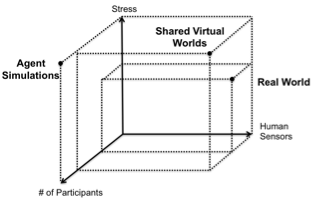
\includegraphics[width=0.30\textwidth]{evaluation-plan.png}}
	\vspace{-3mm} \caption{\small Evaluation using Agent simulations, Shared Online Virtual Worlds, and Real World Experiments.}
	\label{fig1}
	\vspace{-3mm}
\end{wrapfigure}

\subsubsection{Simulation-based Evaluations: Agents. }

The first part of our efforts will focus on developing simulator for the two demonstration settings. Throughout the different phases of the project we will be capitalizing upon ? as well as augmenting the current capabilities of ? the SIDnet SWANS simulator [195] and SteerSuite: The Human Movement and Crowd Simulator [196], being developed at Northwestern and Rutgers respectively. SIDnet is used to evaluate various routing and tracking protocols, shapes detection, and even to evaluate the benefits of high-level programming constructs for WSN-users [113, 160, 187, 191]. SteerSuite is an open-source framework for simulating human movement, deliberation, and is especially geared towards dense crowd situations. We will integrate the functionality of these two systems and further augment them with the capability of having heterogeneous nodes and capturing various mobility models and communications between subsets of such nodes. In addition, we will augment its visualization component as well as introduce a new class of nodes with the proper interfaces to encode the following important features: (1) camera/video/audio based sensing and (2) human and human-operated sensors.  For the multimodal mashup scenario, we will simulate a simplified version of the ?Gold Miner? using computer imagery, with virtual objects and sensors. 
The main use of the simulator in the initial stages of the proposal will be to test the various impacts of uncertainty (sensors, network structure/communication) on the quality of detecting the novel categories of spatio-temporal predicates (cf. Section 3.4) and the impact of different policies for local state-estimation and information extraction (cf. Section 3.1 and 3.3). We will employ a large variety of crowd datasets to train and validate our computational models, and in particular leverage our collaboration with Prof. Dirk Helbing who has significant expertise in crowd data collection, analysis, and modeling [197].  In particular, we will integrate our simulation infrastructure with the NervousNet platform [198] that is being actively developed by Prof. Helbing and his colleagues as part of the larger effort on the Planetary Nervous System project [199], which provides a large-scale distributed research platform for real-time mining of social activities using heterogeneous sensor networks.


\subsubsection{Task E-2. Game Playing Evaluation: Avatars. }

Agent-based simulations, such as those described above provide an efficient way to test and evaluate the different aspects of our system in an automated fashion. However, in an effort to come closer to actual human experimentation, we will conduct experiments using real human users in shared online virtual environments. The Rutgers team is uniquely positioned to conduct these experiments ? Co-PI Kapadia has developed HeapCraft [200, 2001]: a modular, extensible, and open framework for studying human behavior in shared virtual worlds such as Minecraft. HeapCraft has already been successfully demonstrated to study player behavior and incentivize cooperation in online societies [202, 203]. Additionally, Kapadia and his collaborators have also conducted lab experiments to study crowd evacuations using serious games.
We will augment the existing HeapCraft framework to design the two scenarios described in Task E-3 below. HeapCraft?s modular and extensible nature allows us to easily develop emulators for the technologies being developed here, which can be rigorously and robustly tested in shared virtual worlds using real human users. In addition, we will augment the knowledge-base for emulating behavioral aspects of the avatars using large datasets of preferences and semantic relations from real social networks obtained from 4C Insights Inc. (Letter of Commitment is available in the Supplementary Documents). 
Our experiments will be conducted in two phases: (I) laboratory studies where up to 40 participants will be recruited to participate in a controlled experiment; (II) online server with our tools released to setup a virtual world with hundreds of human-users  expected to participate. 


\subsubsection{Task E-3. Real-World Environment Evaluations.  }

XX

 


\section{Broader Impact}\label{broader-impact}
From Rutgers:

The proposed highly interdisciplinary project combines computer vision, human modelling and simulation, optimization, robotics and autonomy, and control theory, and has the potential to impact several research areas. The proposed sensing, simulation, and optimization framework will have wide applicability in various scientific areas involving decision-making in heterogeneous and dynamic networks comprising human-operated, and autonomous sensors, with concepts that could easily generalize to event understanding in complex social, economical or cyber-biological systems, thus impacting multiple societal applications including urban infrastructure, emergency response, safety, and quality of life.

\noindent \textbf{Datasets.} We will release the reconstructed time-stamped behaviors that are collected as part of our real-world experiments in the classroom and the dining hall. This real-world dataset will include both the original, unprocessed, noisy, incomplete trajectories, as well as the processed trajectories for researchers to use and compare, when developing their own algorithms. We will also release synthetic datasets from our simulation experiments using the data-driven crowd simulator that will be developed as part of this research. All crowd datasets (both real and synthetic) will be captured for both the original, un-optimized environments, as well as the optimized layouts. We will also release extended designs actuated of environmental elements such as mobile queue separators and mobile furniture.

\noindent \textbf{Open-Source Software.} The PIs have an established record of releasing software packages related to crowd modeling and simulation ~\cite{steersuite,10.1109/TVCG.2014.251}. We will build on top of these foundations and extend our existing open-source platforms to include software solutions for: (1) crowd trajectory reconstruction, (2) data-driven crowd simulation, (3) static and dynamic analysis of environments, (4) crowd-aware environment optimization, and (5) environment reconfiguration planning.

\noindent \textbf{Kaggle Competitions}. We plan to organize 2 public data analytics competitions using the collected data, hosted on kaggle.com. Kaggle is a platform for predictive modelling and analytics competitions, which is often used in academia to incentivize students to tackle challenging problems through a combination of research, system building, and peer-competitions. The goals will include trajectory estimation and reconstruction, data-driven crowd modelling, and computer-assisted designs of environments.

\noindent \textbf{Curriculum Development and Outreach.} The PIs will generate educational material on the autonomy, hardware design, sensing and simulation aspects of \precise. PI Kapadia will design a graduate seminar on \emph{Crowd-Aware Smart Environments} that will introduce students to concepts in crowd simulation, and environment optimization. Advanced undergraduate students will also be permitted to enroll. PI Pavlovic will introduce an assignment in the machine learning course where students will learn generative models of crowd movement. The PI's will collectively organize a workshop on crowd-aware cyber-physical environments during CPS week (tentatively April 2017), which will bring together researchers from various disciplines including computer vision, machine learning, simulation, robotics, and potential adopters of the technology. Our research environment will provide interdisciplinary training ranging from distributed sensing and control, simulation and optimization, to robot motion planning.

\noindent \textbf{Under-Represented Groups and K-12 Level}. Our project can help attract a diverse group of students and broaden the diversity of students recruited into these and other STEM disciplines. Rutgers office of Enrollment Management conducts the Rutgers Future Scholars Program (RFS), which provides mentoring activities to grade 9-12 minority students from disadvantaged backgrounds and full scholarships to undergraduate programs. We will closely work with this office to participate in outreach, enrichment, and mentoring activities. We will also leverage other programs to recruit and mentor students from under-represented groups: the summer undergraduate Project RiSE (Research in Science and Engineering) for undergraduates from underrepresented populations for 8/1-week intensive summer research internships; and the Aresty Center for Rutgers Undergraduate Research- places Rutgers undergraduates in research laboratories on campus. PI Pavlovic has a multi-year track record of working with over 14 minority and female students through Aresty and RiSE, as well as multiple REUs. We will leverage the extensive diversity programs at Rutgers to recruit and support women and underrepresented minorities.


\section{Results from current and recent prior NSF support}\label{prior-projects}
...

\section{Data management plan}\label{data-management-plan}
....

\section{Project management plan including timeline}\label{project-management-plan}
...\\
...\\ 

\begin{wrapfigure}{R}{0.70\textwidth} \vspace{-3mm}
	\centerline{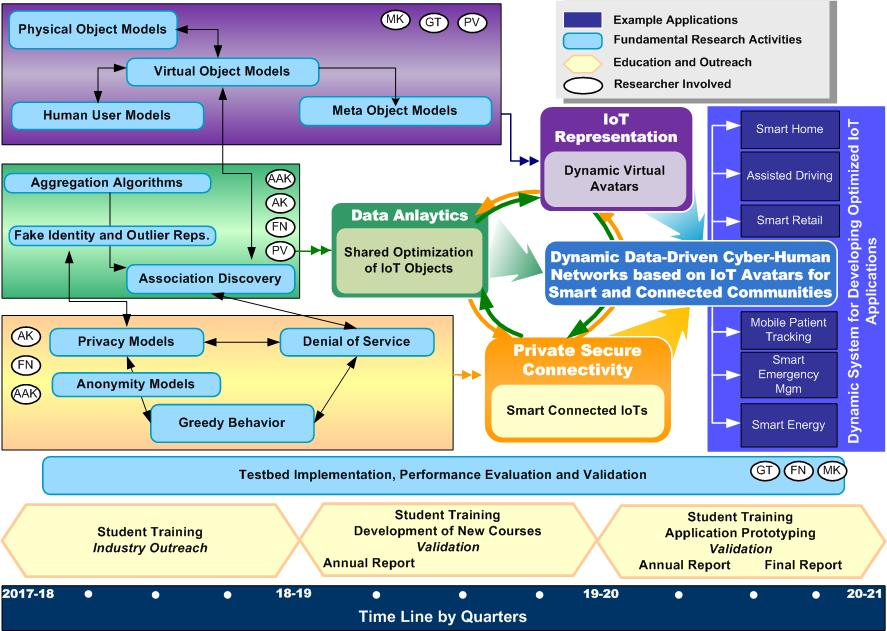
\includegraphics[width=0.61\textwidth]{./Timeline-v1.jpg}}
	\vspace{-3mm} \caption{Collaboration and Deliverables}
	\label{fig8}
	\vspace{-3mm}
\end{wrapfigure}

%%%\newpage

%%%\mypage{M}

%%%\section{Management Plan and Validation}%%
%%%\input{ManagementPlan-v5.tex}
%%%\label{management}

%%%%%%%%%%%Take a look at Phase Transition Phenomena in Wireless Ad-Hoc Networks

\newpage
\mypage{References }

\bibliographystyle{plain}
\bibliography{goce,farid}
%\bibliography{comp11mc-GT-Comprehensive-2011,cps_raf22,pdinda,CPS2012-nikos-12,WSN22,Mokbel,shekhar-refcs,terveen,mining,vipin-references,minnesota-refcs,Prior-bib}

\end{document}
